\section{Two replicas are hard}

In presented model replication is crucial property that makes problems hard. Here we will show that giving minimal replication
possibilities - that is to allow at most 2 replicas of each chunk type - is enough to make problems hard.

\subsection{Idle machines model extension}

We allow spawning more VMs that there are chunk types. Those machines that does not process any chunk still needs to communicate with
other machines.

\subsection{3SAT introduction - NP-completeness of $\CC+\FP+\RS+\BW$}

We prove that $\CC+\RS+\FP+\BW$ is NP-hard by reduction from the Boolean Satisfiability Problem ($\SAT$).
Since $\SAT$ is a decision
problem, we transform $\RS+\FP+\BW$ into a decision problem too, by
introducing a cost threshold $\Thr$.

Let's first recall that the $\SAT$ problem asks whether a positive valuation exists
for a formula $\Formula$ with $\clauses$ clauses and $\variables$ variables.
In the following, we will only focus on $\SAT$ instances of at least four variables;
this problem remains NP-hard.

\textbf{Construction.}
Given any formula $\Formula$ in Conjunctive Normal Form (CNF) with at least four variables, we produce
a $\RS+\FP+\BW$ instance as follows. First, we construct a substrate tree $\Tree_{\Formula}$, consisting of
a root and separate gadgets for each variable of $\Formula$, each of which
is a child of the root.
The gadget of variable $\variab$ has a root, $\aroot(\variab)$, and two children:
$\positive(\variab)$ and $\negative(\variab)$. Child $\positive(\variab)$ has $\clauses$
many children $v_1, v_2, \ldots, v_{\clauses}$, and child $\negative(\variab)$ has
$\clauses$ many children $\neg v_1, \neg v_2, \dots, v_{\clauses}$. Every
gadget has the same structure: the same height and the same number of
leaves. By default, we will set the available bandwidth to be the
same everywhere, in every gadget; differences will be shown when we
will place chunks.

We set the number of virtual machines to $\Vms = \clauses \cdot \variables$.
Moreover, we define the inter-connect communication cost to be $1$,
and the access cost to be a sufficiently large constant $W$,
such that nodes must always be collocated with chunks.
(For a concrete value, use $W=$TODO).


We set the following bandwidth capacities in the substrate. There are three
levels of edges in the substrate network $\Tree_{\Formula}$ given by formula
$\Formula$: \emph{top}, \emph{middle} and \emph{bottom}.
We do not consider any capacities at the \emph{bottom} and \emph{middle} levels.
At a top-level edge, we set the bandwidth to $\clauses \cdot (\variables -
\clauses)$.

We set the number of chunks to be equal to the number of clauses, $\ChunkTypes =
\clauses$. To finish our construction, we place data chunks at
leaves, as follows: for the $i$-th clause we
construct as many replicas of chunk $\achunk_i$ as there are literals in the
clause. For each literal $\ell$ (of the form $\variab$ or $\neg \variab$) that satisfies clause $i$ we place
replica of chunk $\achunk_i$ in the leaf labeled $\achunk_{\ell_i}$.

The threshold $\Thr$ is given by the
communication cost among nodes in
a certain solution to our instance. This solution is constructed by embedding
nodes at all leaves of $\positive(\variab)$ and none at leaves
$\negative(\variab)$, for every gadget of variable $\variab$. Please note that $\Thr$
computed in such a way does not contain transportation cost. TODO: calculate
$\Thr$.

\textbf{Proof of correctness of construction.}
With our construction completed, we need to prove that it indeed
decides $\SAT$. We set the capacities such that in every gadget,
at most $\clauses$ nodes can be spawned, where $\clauses$
is the number of clauses of $\Formula$.
We can apply the Bandwidth Lemma (Lemma~\ref{lem:bandwidth-lemma}) as follows:
We interpret $a_i$ as the
number of nodes that are embedded in the $i$-th gadget, $\clauses$
as the number
of clauses and $\variables$ as the number of variables.
The LHS of the inequality of Lemma~\ref{lem:bandwidth-lemma}
is a formula for the communication cost of nodes inside the $i$-th
gadget to nodes outside the gadget. The RHS of the inequality is the
bandwidth constraint for the gadget. This implies that
any feasible solution must embed exactly $\clauses$ nodes in every gadget.


\begin{theorem}
The problem $\RS+\FP+\BW+\CC$ is NP-hard.
\end{theorem}
\begin{proof}
We will prove that formula $\Formula$ is satisfiable iff $\RS+\FP+\BW+\CC$ has
a solution of cost $\leq \Thr$.

($\Rightarrow$) Let us take any valuation $\Val$ that satisfies $\Formula$.
We will construct a solution to $\RS+\FP+\BW$ using $\Val$ in the following way.
For each variable $\variab$ in $\Formula$, we embed $\clauses$ many nodes
at the  leaves of the gadget of $\variab$. We need to choose $\clauses$ out of
$2 \cdot \clauses$ leaves to embed nodes. If $\Val(\variab) = 1$, we embed
nodes at the leaves
of $\positive(\variab)$, else we embed all nodes at leaves $\negative(\variab)$.
The solution constructed this way has cost exactly
$\Thr$, because the nodes are evenly split among gadgets, and nodes are not
distributed across $\positive(\variab)$ and $\negative(\variab)$ subtrees.

We calculate the chunk-node matching $\mu$ by assigning every chunk to
the node which is collocated with the first chunk replica. This solution is feasible
(every chunk type is processed),
because the given valuation satisfied $\Phi$.

Now we will show that this solution has cost $\Thr$.
Due to the Bandwidth Lemma (Lemma~\ref{lem:bandwidth-lemma}),
we only have to consider the communication cost.

($\Leftarrow$) Let us take any solution to $\RS+\FP+\BW$ constructed based on $\Formula$ of cost $\leq \Thr$.
We will construct a positive valuation $\Val$ by considering the nodes in
the solution to $\RS+\FP+\BW$.

We make the following observations. In every solution of cost
$\leq \Thr$, every gadget has exactly $\clauses$ many nodes
at its leaves. This is due to the Bandwidth Lemma (Lemma~\ref{lem:bandwidth-lemma}).
Also, inside
every gadget either all nodes are in the $\positive(\variab)$ subtree
of variable $\variab$, or in the $\negative(\variab)$ subtree. This is true
because the cost of a solution where at least one gadget has nodes
distributed across subtrees is
always greater than $\Thr$.

TODO Maciek: prove it more formally. First, define semi-feasible solution. Let's take any $p,q$ being the number of nodes
spawned in left and right subtree. Then we say that we can improve the
solution by moving all $q$ to where $p$s lie and we have cheaper solution.

Now we can construct our valuation $\Val$, as follows
(for each variable $\variab$ in $\Formula$):
If $v_1$ hosts a node then $\Val(\variab) = \top$,
otherwise $\Val(\variab) = \bot$.

The valuation $\Val$ satisfies all clauses, and hence $\Formula$,
as the solution to $\RS+\FP+\BW$ covers all chunks. To see this,
consider the leaf handling any given clause chunk;
it is a witness that the corresponding clause is true.
\end{proof}

\subsection{Two replicas are hard ($\RS(2)+\FP+\CC+\BW$)}\label{ssec:two}

Our results so far indicate that dealing with replication can be challenging.
However, all our hardness proofs concerned scenarios with three replicas,
which raises the question whether the problems can be solved in polynomial time
with a replication factor of two only. (Similarly to, say, the $\ZSAT$ problem
which is tractable in contrast to $\TSAT$.)

In the following, we show that this is not the case: the problem remains
NP-hard, at least in the capacitated network.

The proof is by reduction from $\TSAT$. Given a formula $\Formula$ in
conjunctive normal form, consisting of $\clauses$ clauses and $\vars$ variables, we construct a problem instance and substrate tree
$T_{\Formula}$ using two types of gadgets: gadgets for variables and
gadgets for clauses. \emph{Nota bene:}
unlike in the previous proofs, for every clause we will create three chunk types instead of just one.

\textbf{Construction.}
We distribute chunks among servers as follows. First,
similarly to the previous proofs with three replicas, we put clause chunks in
variable gadgets; however, now we place distinct chunks instead of
three copies of the same chunk. Second, we place three chunks that
correspond to clauses in all three leaves of their clause gadgets.
Thus, in total, $6 \cdot \clauses$ variable chunks are mapped.
We will consider a setting where $cv + 2\clauses$ nodes \stefan{what is $cv$ here?} need to be mapped. Our intention is that in
every variable gadget, there will be $\clauses$ nodes,
 and in every clause
gadgets there will be two nodes.

The available bandwidth of the top edge of the gadget of each variable $\variab$ is set to
$\capa(v) = 3  \cdot  3  \cdot  (3  \cdot  (\vars - 1) + 2  \cdot  \clauses) $.
The first factor is the tree distance which is 6 divided by 2 (as
we count each pair twice). The second factor is
the number of nodes to be placed in every variable gadget.
So the first term of the
sum is three times the number of outer variable gadgets,
and the second term is the
number of nodes in each of the $\clauses$ clause gadgets.

The available bandwidth for the top edge of each clause gadget is set to
$\capa(\clauses) = 3  \cdot  2  \cdot  (2  \cdot  (\clauses - 1) + 3  \cdot  \vars) $.

\stefan{TODO Carlo: The construction is illustrated in Figure~\ref{fig:two}.}


\textbf{Proof of correctness.}
We first prove the following helper lemma.
\begin{lemma}
Every valid solution to $\FP+\RS(2)+\BW+\CC$
with cost at most $\Thr$ has the property that
there are exactly $\clauses$ nodes in each of the $\vars$ variable gadgets
and exactly two nodes in each of the $\clauses$ clause gadgets.
\end{lemma}
\begin{proof}
The claim is due to the bandwidth constraints. We have to take into
consideration the following communication paths:
communication to clause gadgets and
communication to
other variable gadgets.
In every valid solution of cost at most $\Thr$ we have exactly
$\clauses$ nodes in each variable gadget and two nodes in each clause gadget.
\end{proof}

\begin{theorem}
$\FP+\RS(2)+\BW+\CC$ is NP-hard.
\end{theorem}
\begin{proof}
We show that $\FP+\RS(2)+\BW+\CC$ has a solution of cost $\leq
  \Thr$ if and only if $\Formula\in \TSAT$ is satisfiable.

($\Rightarrow$) If we have a positive valuation of $\Formula$, we fill variable gadgets with nodes like in
the proofs before. Then we fill $2 \cdot \clauses$ nodes as follows:
\begin{itemize}
\item If the first literal satisfies the clause, we map two nodes in the second and
third leaf of the corresponding clause gadget.
\item If the first literal does not satisfy the clause, we map two nodes to the first
and second leaf of the clause gadget.
\end{itemize}

TODO: chunk assignment should be based on valuation!

We then assign chunks to nodes as follows:
\begin{itemize}
\item Chunk $\achunk_i^1$ is matched to the node which is located in a variable gadget; there
must be one, as the valuation satisfies the formula.
\item Chunks $\achunk_i^2$ and $\achunk_i^3$ are matched to nodes which are
located in clause
gadgets; there exist corresponding minimal-cost solutions.
\end{itemize}

Thus, we have produced a feasible solution of cost $\Thr$, as there are no
access and inter-connect costs.

($\Leftarrow$)
Let us take any solution $\Sol$ to $\RS(2)+\FP+\BW$ of cost $\leq \Thr$.
Then we can compute a positive valuation by setting each variable $\variab$
as follows:
$\Val(\variab)= \top$ iff there is a node at the first leaf on the positive side of the $\variab$ gadget in $\Sol$,
and $\Val(\variab)=\bot$ otherwise.

%$\Val(\variab)$ =
%\begin{cases}
%\top & \mbox{iff there lies VM on first leaf on positive side of $\variab$ gadget in $\Sol$}\\
%\bot & \mbox{otherwise}
%\end{cases}

The theorem now follows from the following two additional lemmas.
\begin{lemma}
For every clause there exists a node in a variable gadget that processes one of
  three chunks that correspond to that clause.
\end{lemma}
\begin{proof}
 Each of the three chunks that correspond to every clause,
 is assigned a collocated node.
 At least one of those three nodes is not idle in a variable gadget;
otherwise, those two VMs in clause gadgets would not suffice in
satisfying all chunk types.
\end{proof}

Observation. It might happen that in $\Sol$, two nodes in
clause variables are idle, and three nodes in variable gadgets are
processing those $3$ chunk types. In this case, we
arbitrary nodes can be taken in the rest
of the proof.

\begin{lemma}
$\Val$ satisfies $\Formula$.
\end{lemma}
\begin{proof}
Let us consider the matching $M$ of $\Sol$, and let us consider an arbitrary clause of
$\Formula$ as well as its $3$ chunk types: $\achunk_i^1, \achunk_i^2, \achunk_i^3$.
We will refer to the nodes corresponding to them
by $v_i^1, v_i^2, v_i^3$; two of them lie in clause gadgets.
Take the chunk type that was processed in variable
gadgets and look at where it was processed.
In our valuation $\Val$, we set the literal of the node leaf to
$\top$; therefore the clause is satisfied.
\end{proof}
\end{proof}

\subsection{SAT bandwidth lemma proof}
The following lemma is useful in our NP-hardness proofs.

\begin{lemma}[Bandwidth Lemma]\label{lem:bandwidth-lemma}
  Let $\clauses$ and $\variables > 4$ be two arbitrary positive integers. Let $a_1, a_2, \ldots,
  a_{\variables}$ be a sequence of $\variables$ integers which adds up to $\clauses \cdot \variables$. Also, for
  each $i$ we have $a_i \leq 2 \cdot \clauses$. Then it holds that if
  $$ \forall_i:~~ a_i \cdot (\clauses \cdot \variables - a_i) \leq \clauses \cdot (\clauses \cdot \variables -
  \clauses), $$
\noindent  then for each $i$: $a_i = \clauses$.
\end{lemma}
\begin{proof}
For the sake of contradiction, let us assume that there exists an index $k$ such that
$a_k \neq \clauses$. Then we can distinguish between two cases:
either $a_k<\clauses$ or
$a_k>\clauses$.

\textbf{Case $a_k<\clauses$:} If there exists a $k$ with $a_k<\clauses$,
due to the fact that the sequence adds up to $\clauses \cdot \variables$,
there must also exist a $k'$ such that $a_{k'}<\clauses$ (by a simple
pigeon hole principle). Thus, this case can
also be reduced to the second case (\textbf{Case $a_k>\clauses$}) proved
next.

\textbf{Case $a_k>\clauses$:} Since it also holds that $a_k < 2\clauses$,
$a_k$ must be of the form $\clauses + x$ for $x \in [1, \ldots, \clauses]$.
Let us consider the (bandwidth) inequality:
$$ (\clauses + x) \cdot (\clauses \cdot \variables - \clauses - x) \leq \clauses \cdot (\clauses \cdot \variables - x) $$

This can be transformed to:

$$ 0 \leq x(x - (\clauses \cdot (\variables - 2))) $$

The equation holds for $x \leq 0$ or $x \geq \clauses \cdot (\variables - 2)$,
and no
positive $x \leq \clauses$ can satisfy this inequality for $\variables > 4$. Contradiction.
\end{proof}


\subsection{Images}

\begin{figure}[htbp]
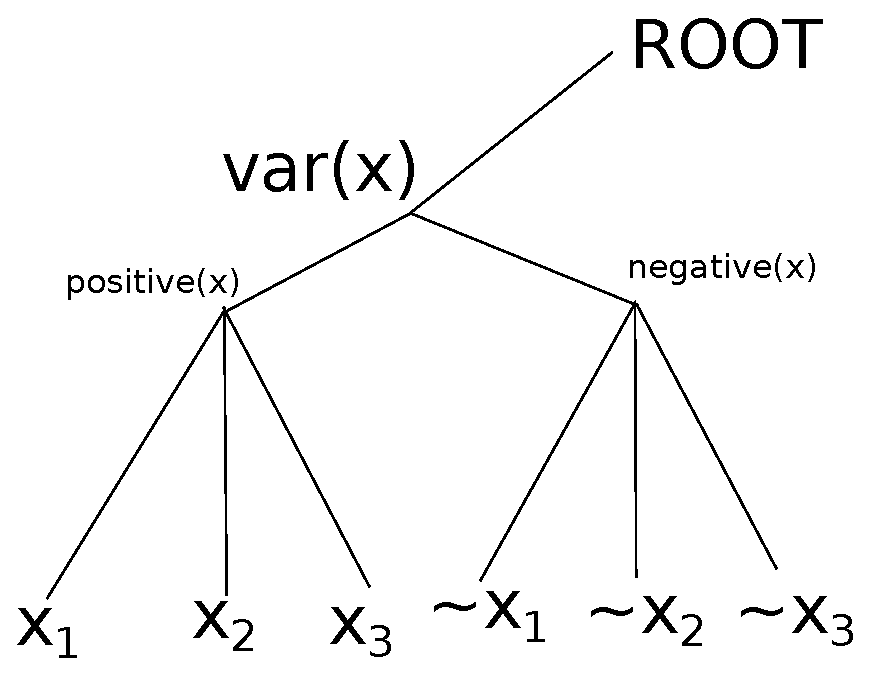
\includegraphics[width = \columnwidth]{figs/gadget-no-bw}
\end{figure}


\begin{figure}[htbp]
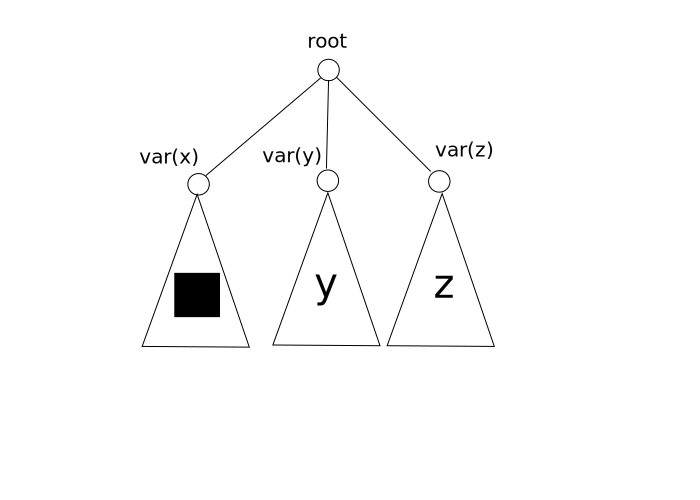
\includegraphics[width = \columnwidth]{figs/vc-instance}
\end{figure}


\begin{figure}[htbp]
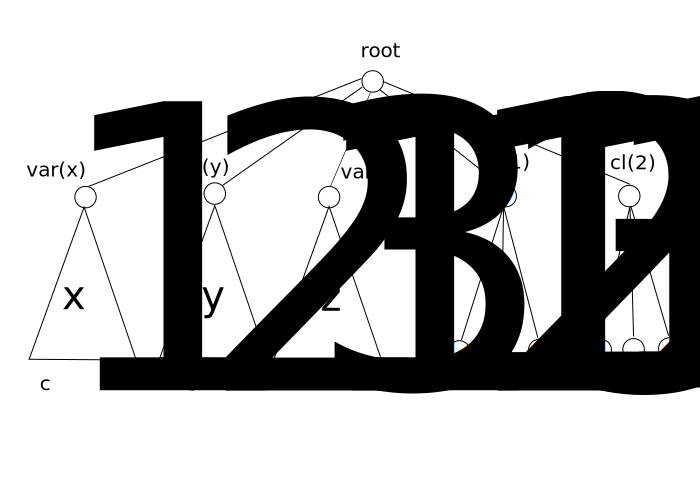
\includegraphics[width = \columnwidth]{figs/vc-instance-r2}
\end{figure}


\begin{figure}[htbp]
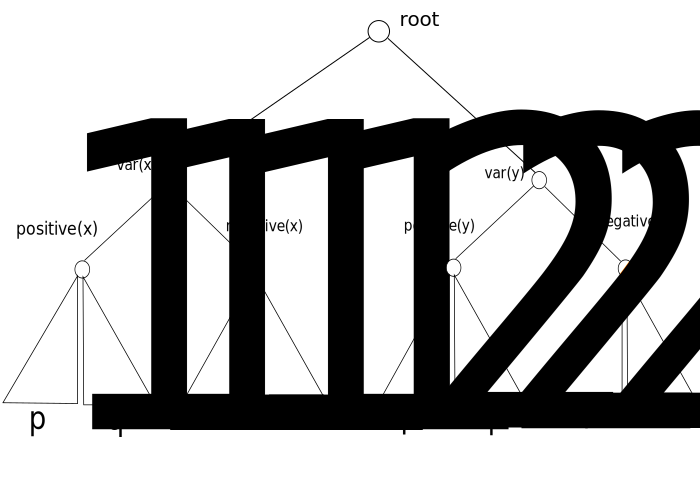
\includegraphics[width = \columnwidth]{figs/lemma-two-gadgets}
\end{figure}


\begin{figure}[htbp]
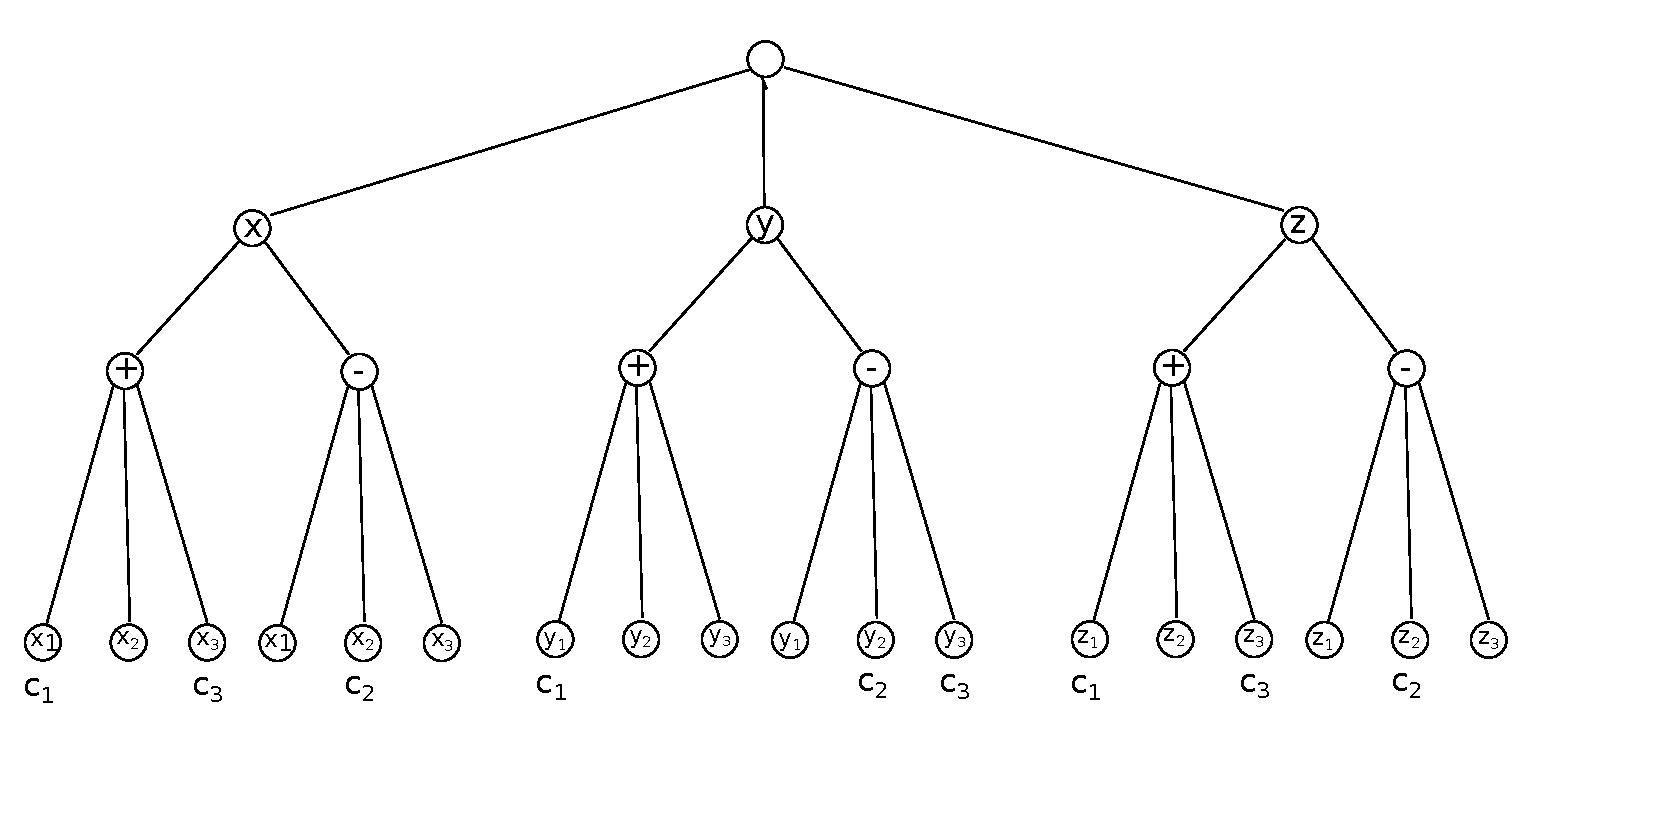
\includegraphics[width = \columnwidth]{figs/formula-example}
\end{figure}


